\documentclass[11.5pt]{sig-alternate} % sets document style to sig-alternate
% packages
% typesetting
%\usepackage{dirtytalk} % typset quotations easier (\say{stuff})
\usepackage{hanging} % hanging paragraphs
\usepackage[defaultlines=3,all]{nowidow} % avoid widows
\usepackage[pdfpagelabels=false]{hyperref} % produce hypertext links, includes backref and nameref
\usepackage{xurl} % defines url linebreaks, loads url package
\usepackage{microtype}
%\usepackage[super]{nth} % easily create superscript ordinal numbers with \nth{x}
\usepackage{textcomp}
\newcommand{\texttildemid}{\raisebox{0.4ex}{\texttildelow}}
% layout
%\usepackage{enumitem} % control layout of itemize, enumerate, description
\usepackage{fancyhdr} % control page headers and footers
\usepackage{float} % improved interface for floating objects
%\usepackage{multicol} % intermix single and multiple column pages
% language
\usepackage[utf8]{inputenc} % accept different input encodings
\usepackage[english]{babel} % multilanguage support
% misc
\usepackage{graphicx} % builds upon graphics package, \includegraphics
%\usepackage{lastpage} % reference number of pages
%\usepackage{comment} % exclude portions of text (?)
\usepackage{xcolor} % color extensions
\usepackage[backend=biber, style=apa]{biblatex} % sophisticated bibliographies % necessary for HTML to display author info and date on abstract page
\usepackage{csquotes} % advanced quotations, makes biblatex happy
\usepackage{authblk} % support for footnote style author/affiliation
% tables and figures
\usepackage{tabularray}
%\usepackage{array} % extend array and tabular environments
\usepackage{caption} % customize captions in figures and tables (rotating captions, sideways captions, etc)
%\usepackage{cuted} % allow mixing of \onecolumn and \twocolumn on same page
\usepackage{multirow} % create tabular cells spanning multiple rows
%\usepackage{subfigure} % deprecated, support for manipulation of small figures
%\usepackage{tabularx} % extension of tabular with column designator "x", creates paragraph-like column whose width automatically expands
%\usepackage{wrapfig} % allows figures or tables to have text wrapped around them
%\usepackage{booktabs} % better rules
% dummy text
%\usepackage{blindtext} % blind text dummy text
%\usepackage{kantlipsum} % Kant style dummy text
\usepackage{lipsum} %lorem ipsum dummy text
% other helpful packages may be booktabs, longtable, longtabu, microtype

\pagestyle{fancy} % sets pagestyle to fancy for fancy headers and footers

% header and footer
% modern way to set header image
\renewcommand{\headrulewidth}{0pt} % defines thickness of line under header
\renewcommand{\footrulewidth}{0pt} % defines thickness of line above header
\setlength\headheight{80.0pt} % sets height between top margin and header image, effectively moves page contents down
\addtolength{\textheight}{-80.0pt} % seems to affect the lower height. maybe only works properly if footer numbers enabled?
\fancyhf{}
\fancyhead[CE, CO]{
\includegraphics[width=\textwidth]{headerImage.png}}
% footer
%\fancyfoot[LE,LO]{Article Title Here \\ DOI: }% left footer article title and doi
%\fancyfoot[CE,CO]{{}} % center footer empty
%\fancyfoot[RE,RO]{\thepage} % right footer page numbers
%\pagenumbering{arabic} % arabic (1, 2, 3) numbering in footer

\hypersetup{colorlinks=true,urlcolor=blue} % sets link color to blue
\urlstyle{same} % sets url typeface to same as rest of text

% set caption and figure to italics, label bold, left align captions, does not transfer to HTML
\DeclareCaptionFormat{custom}
{
    \textbf{\textit{\large #1#2}}\textit{\large #3} % #1 is the "Table 1" or "Figure 1" part, #2 is the separator (":"), #3 is the caption
}
\captionsetup{format=custom}
\captionsetup{justification = raggedright, singlelinecheck = false}

%this next bit is confusing, but essentially changes the width of the abstract. Seems to have been copied from this https://tex.stackexchange.com/questions/151583/how-to-adjust-the-width-of-abstract
\let\oldabstract\abstract
\let\oldendabstract\endabstract
\makeatletter %changes @ catcode to enable modification (in parsep)
\renewenvironment{abstract} %alters the abstract environment
{\renewenvironment{quotation}%
               {\list{}{\addtolength{\leftmargin}{1em} % change this value to add or remove length to the the default ?
                        \listparindent 1.5em%
                        \itemindent    \listparindent%
                        \rightmargin   \leftmargin%
                        \parsep        \z@ \@plus\p@}%
                \item\relax}%
               {\endlist}%
\oldabstract}
{\oldendabstract}
\makeatother %changes @ catcode to disable modification

% checks
% italics 
% links -
% dashes -
% tildes - 
\begin{document}

\title{Teachers’ Perception of an Integrated Approach to Biology and Emotional Learning}

\author[1]{\large \color{blue}Laura Ferreira González}
\author[1]{\large \color{blue}Thomas Hennemann}
\author[1]{\large \color{blue}Kirsten Schlüter}
\affil[1]{University of Cologne}

\toappear{}
%% ABSTRACT
\maketitle
\begin{@twocolumnfalse} 
\begin{abstract}
\item 
\textit{Inclusive education requires that teachers not only teach academic knowledge and skills, but also consider the individual needs of all pupils, especially with respect to their social-emotional status. All teachers (including science and biology teachers) have to promote the wellbeing of their pupils by helping them develop social-emotional skills. The positive impact of these skills has been widely researched and documented. There is no doubt that academic achievements and social-emotional skills go hand in hand. However, only very little research data are available on how biology lessons and biology teachers can facilitate inclusive education in everyday school. The purpose of this qualitative study is to find out how teachers perceive an integrated approach in biology classes. This study reports on the experiences of five biology teachers with an integrated approach in which learning about the human body was intertwined with socio-emotional learning to address all pupils’ needs. Overall, the teachers considered the use and implementation of the approach a success. They observed that the pupils were motivated and showed a high level of active involvement and participation. However, it became obvious that the teachers did not fully realize all elements of the approach—the intertwined biological and emotional learning in particular—although they liked it. Finally, our findings show that a practical way to teach science and emotional learning can be realized in common, but teachers need further support and professional development.}
\\ \\
Keywords: human biology education, inclusive learning, social emotional skills, teachers’ perception
\end{abstract}
\end{@twocolumnfalse}

%% AUTHOR INFORMATION

\textbf{*Corresponding Author, Laura Ferreira González}\\
\href{mailto: l.ferreiragonzalez@uni-koeln.de }{(l.ferreiragonzalez@uni-koeln.de)} \\
\textit{Submitted November 1st, 2018 }\\
\textit{Accepted January 31, 2019} \\
\textit{Published online April 9th, 2019} \\
\textit{DOI: 10.14448/jsesd.11.0002} \\
\pagebreak
\clearpage

\begin{large}
\section*{INTRODUCTION}
    
As a result of the ratification of the UN Convention on the Rights of Persons with Disabilities, each country is required to implement inclusive education by offering equal access to all pupils in primary and secondary school (United Nations, 2006). In Germany, where this study took place, the transition from a segregated or excluding education system to an inclusive education system is still in progress (Ministerium für Schule und Bildung des Landes Nordrhein-Westfalen, 2018). Pérez-Parre\~no and Padilla-Petry (2018, p. 189) describe inclusive education as “a process that seeks to embrace all pupils, recognizing their particularities, valuing them all and giving them the chance to participate in school in accordance with their abilities” (cf. Thomazet, 2009; Vislie, 2003). Inclusive classes are characterized by the diversity of the pupils, regarding, but not limited to, social background, ethnicity, disability, and gender (cf. Georgi, 2015). Teachers in inclusive classes face a variety of challenges, especially when it comes to pupils who have shortcomings in emotional and social skills (Gidlund \& Boström, 2017).

\section*{THEORETICAL BACKGROUND}
\subsection*{Teachers' Challenges in Inclusive Classrooms}

Teachers in inclusive classrooms face challenges as diverse as the pupils they teach. Forlin, Keen, and Barrett (2008) identified pupils’ behavior and teachers’ self-perceived lack of professional competences as the two main fields of teachers’ concerns in inclusive classrooms. Difficult behavior includes short attention span, poor communication skills, and inappropriate social skills for example (Forlin et al., 2008). Pupils with behavioral problems are particularly challenging (Kyriacou, 2009; Wilson, 2002). Teachers’ concerns include the lack of appropriate resources and support, large class sizes, insufficient pre- and in-service training, and difficulties in monitoring other pupils while attending to the student with special needs (Forlin et al., 2008; Klassen \& Anderson, 2009; Martin, Linfoot, \& Stephenson, 1999; Wagner et al., 2006). Only a few special teacher education programs focus on or address classroom or behavior management explicitly (Oliver \& Reschly, 2010). About half of the courses in general teacher preparation programs deal with classroom management, which are most common in elementary programs (J. Greenberg, Putman, \& Walsh, 2014). Fewer programs (about one third) include practical learning opportunities. Keeping the attention of pupils with behavioral problems focused on the learning subject is far from easy (Lamport, Graves, \& Ward, 2012), as due to the relatively large number of pupils in regular class (20-30 pupils), there is only little time to support and monitor pupils with special needs (Arbeiter \& Hartley, 2002; Conderman, 2011; Talmor, Reiter, \& Feigin, 2005). This might explain why schools are generally rather reluctant to accept pupils with disruptive behavior and educational and behavioral disorders (EBD; Visser \& Stokes, 2003). For example, in Germany, schools are still not (legally) obligated to accept all children, especially those with special needs.

\subsection*{Situation of Inclusive Classes in Grades Five and Six}

Pupils in grades five and six (10- to 12-years-olds in Germany) are in transition from middle childhood to early adolescence (Berk \& Meyers, 2015). This phase of development is characterized by different processes of separation. For example, peers become the relevant reference group instead of the family. Furthermore, pupils at this age have just left primary school (at the end of grade four) and entered secondary school in most states of Germany. This transition can cause stress as the pupils need to find new friends and have to get along with new and different teachers as well as adapt to a new environment (Berk \& Meyers, 2015). This stress can cause psychosocial difficulties, especially in pupils with special education needs (Hughes, Banks, \& Terras, 2013). However, all pupils at this age have to learn to replace maladaptive strategies of emotional regulation (such as confrontation, aggression, ignorance, and self-reproaches) by adaptive strategies (such as explanation, reconciliation, humor, and palliative emotion regulation; Salisch \& Vogelgesang, 2005). The challenge for teachers is to support the development of their pupils’ emotional competences. There is a variety of ways and methods to do so.

\subsection*{A Possible Solution}

Teachers are crucial when it comes to pupils’ emotional development. Jennings and Greenberg (2009) suggest that teachers, who consider themselves socially and emotionally competent, can create a classroom environment that enhances the intrinsic motivation of their pupils and improves the skills of cooperation and age-appropriate regulation strategies. The prosocial classroom model by Jennings and Greenberg (2009) explains how teachers’ social-emotional competences, effective classroom management (CM), and effective social and emotional learning (SEL) implementation work together to contribute to a healthy classroom environment that fosters the academic and social-emotional achievements of all pupils alike. This and other models on SEL (M. T. Greenberg, Domitrovich, Weissberg, \& Durlak, 2017) and CM (Helmke \& Helmke, 2015) imply that effective CM and SEL are not limited to a particular group like EBD pupils. In fact, both can support all pupils in their personal developmental processes. 

\subsubsection*{Classroom Management} 

A precondition for a healthy personal development of pupils is a safe learning environment (Nash, Schlösser, \& Scarr, 2016; Reicher, 2010), which can be achieved through effective CM. Classroom management is defined by Evertson and Weinstein (2006, p. 4) as “the actions teachers take to create an environment that supports and facilitates both academic and social-emotional learning.” One possible element of CM is establishing rules and routines by introducing them in the first lesson or developing them together with the students (Emmer \& Evertson, 2013). The pupils then know the rules and routines in class. Effective CM promotes a trustworthy and respectful relationship between teachers and pupils. Several studies in regular schools, inclusive schools, and special schools have proven that effective classroom management has positive effects on pupils’ academic learning, social-emotional development, and learning and working behavior (Hutchings, Martin-Forbes, Daley, \& Williams, 2013; Korpershoek, Harms, de Boer, van Kuijk, \& Doolaard, 2016).

\subsubsection*{The Relevance of Social and Emotional Learning (SEL)} 

Social and emotional learning (SEL) is defined by The Collaborative for Academic, Social, and Emotional Learning (CASEL, 2017) as the
\begin{quote}
    process through which children and adults acquire and effectively apply the knowledge, attitudes, and skills necessary to understand and manage emotions, set and achieve positive goals, feel and show empathy for others, establish and maintain positive relationships, and make responsible decisions (CASEL, 2017).
\end{quote}

SEL can support pupils with psychosocial disorders and EBD by equipping them with necessary skills. With a focus on SEL, pupils can learn how they can cope with everyday life challenges. Social-emotional competences (SEC; e.g., identification of emotions in themselves and others, the ability to manage one’s own emotions, and the development of positive interactions) and the different ways they can be taught in schools have been a broad field of study (Elias et al., 1997; Reicher, 2010; Schwab \& Elias, 2015). International meta-analyses have confirmed the effectiveness of SEL on prosocial behavior, the reduction of antisocial behavior, and academic achievement, among other things (Durlak, Weissberg, Dymnicki, Taylor, \& Schellinger, 2011; Sklad, Diekstra, De Ritter, Ben, \& Gravesteijn, 2012). Akelaitis and Lisinskiene (2018) summarize several studies of the advantages of promoting SEC, such as better school performance, relationships of higher quality, the ability to solve social problems more effectively, and less unhealthy behavior. Oberle (2018) describes a positive effect of SEL on peer acceptance in early adolescence as well.

\subsubsection*{The Role of Teachers} 

In contrast to these general studies, little is known about how biology teachers perceive SEL as tool to facilitate inclusion. This is of relevance as teachers play an important role in the implementation, efficacy, longevity, and effectiveness of SEL programs (Humphries, Williams, \& May, 2018). Teachers seem to be aware of their crucial role, as they state that “teaching entails supporting the social-emotional development of pupils” (Humphries et al., 2018, p. 167) and goes “far beyond the school age” (Humphries et al., 2018, p. 167). While teachers accept SEL as an important lesson objective, an earlier study found that less than half of teachers had implemented SEL programs in their classes (Buchanan, Gueldner, Tran, \& Merrell, 2009). The main reasons mentioned by teachers for engaging in SEL were problems in pupils’ behavior and academic performance, rather than simply to support all pupils’ learning through best practices. Thus, “schools often engage in interventions that are reactive rather than proactive” (Buchanan, Gueldner, Tran, \& Merrell, 2009, p. 188). However, there is increasing awareness that SEL might be as important as learning basic competences like reading and mathematics (M. T. Greenberg et al., 2003).

\section*{RESEARCH QUESTIONS}

In Germany, as in all countries in which the UN Convention (United Nations, Convention on the Rights of Persons with Disabilities, Vereinten Nationen, 2008) was ratified, establishing a fully inclusive education system still requires time and effort. The main challenge seems to be the contrast between the statutory provisions and everyday teaching. However, legislation requires that teachers assume responsibility for the physical and mental well-being of their pupils, including SEL. Education is thus no longer limited to the teaching of subject matter even though this is what many teachers still focus on, especially as they do not feel prepared for teaching inclusively. For biology teachers, this means that many of them want to teach biology first and foremost. However, the diversity of the pupils and the different challenges that teachers face every day make it clear that biology lessons cannot be limited to academic learning but also must include SEL. A way to support teachers is to show them how SEL, CM, and subject content can be taught together. At present, little is known about teachers’ perceptions of such an approach (cf. Humphries et al., 2018).

This study investigates the following questions: How do biology teachers perceive an inclusive teaching approach in biology class integrating learning about the human body, emotional learning, and classroom management strategies? What are their experiences? What do they notice in terms of the academic performance and the social-emotional competences of their pupils?

\section*{METHOD}

\subsection*{The Teaching Approach: Programmed Teaching Series Plan for Biology Lessons}

To answer these research questions, we developed an inclusive teaching approach bringing together learning about the human body, SEL, and CM. This approach was operationalized by a programmed teaching series plan for biology lessons (Inclusive Biology Education [IBE]; Ferreira González, Leidig, Hennemann, \& Schlüter, 2016). The series consists of 23 biology lessons, which weave together learning about the human body and SEL. All lessons include pro- and reactive strategies of effective CM (Emmer \& Evertson, 2013). Table 1 gives an overview of these strategies and their practical implementation in the lessons. 

\begin{table*}[thbp]
\caption{Implementation of Classroom Management Strategies within the Intervention}
\begin{tabular}{ll}
\hline
Strategy & Implementation of the strategy within the intervention \\ \hline
Organizing classroom and materials & The organization of the classroom and of the material includes the adjustment of the seating plan, which means that every pupil has a direct view to the teacher and the teacher has a direct view to every student. Necessary teaching materials are easily accessible for the teachers as well as for all pupils. Posters with relevant information are visible during the lessen, e.g. classroom rules (see below) and the lesson overview. \\
Establishing classroom rules and procedures & Three rules are agreed upon by the teacher and the pupils in advance and are repeated at the beginning of each lesson and if needed. The three rules are: (a) I raise my hand when I want to say something. (b) I listen and participate. (c) We are kind to each other. Learners know and understand what rules apply and what behavior is expected of them in the classroom and under particular conditions, and in open learning situations in particular. \\
Defining consequences & A token reward system is established, i.e. every pupil receives feedback at the end of each lesson in form of thumb stamps. Thumb stamps are awarded depending on whether each student grasps the biological and emotional learning scopes. In addition, individual feedback for three selected pupils per lesson is given. Teachers reinforce the positive behavior of pupils and establish consequences for situations in which rules and procedures are disregarded. \\
Getting off to a good start & A positive learning atmosphere supports pupils' learning. Teachers and students are encouraged to be polite and respectful towards each other and to show willingness to collaborate. \\
Withitness and overlapping & Pupils are highly involved through the use of different learning activities, e.g. quizzes, random selection of pupils for questions. The teacher is always aware of what is going on in the classroom, which includes changing positions in the room depending on the situation. \\
Appropriately prepared lessons & The teachers familiarize themselves with the theoretical basis of the teaching unit/the course plans/prefabricated working material for all students and adjusts the materials to the pupils' learning preconditions. \\
Procedures for managing students’ work & The pupils are active participants in the teaching process. Among other things, this can improve the self-efficacy abilities of the learners. The pupils use support- and self-assessment cards to support and evaluate their learning process. Pupils are responsible for rotationally switching special tasks they have taken over in a lesson, like acting as a time guard or assisting in distributing the learning materials. \\
Planning and conducting instruction & The teacher makes the course of the lesson and its objectives transparent to his/her pupils by naming this information and making it visible on the chalkboard. Every lesson follows the same sequence of introduction, practice, and closure. \\
Managing cooperative learning groups & The teacher uses cooperative learning methods, e.g. think-pair-share, jigsaw), to promote positive interdependence, which means that group members receive different tasks/materials but must pursue a common goal, which they can only reach through cooperation. \\
Managing problem behaviors & The teacher applies various reactive strategies in case of inadequate behavior like making eye contact or giving humorous feedback. \\ \hline
\end{tabular}
\end{table*}

The topic of the human body was selected, as it is one of the key topics in curriculum guidelines for these particular grades (MSW Ministerium für Schule und Weiterbildung Nordrhein-Westfalen, 2013) and the subject- and emotional-oriented lesson content can be easily connected with each other (see Figure 1). 

\begin{figure*}[!h]
    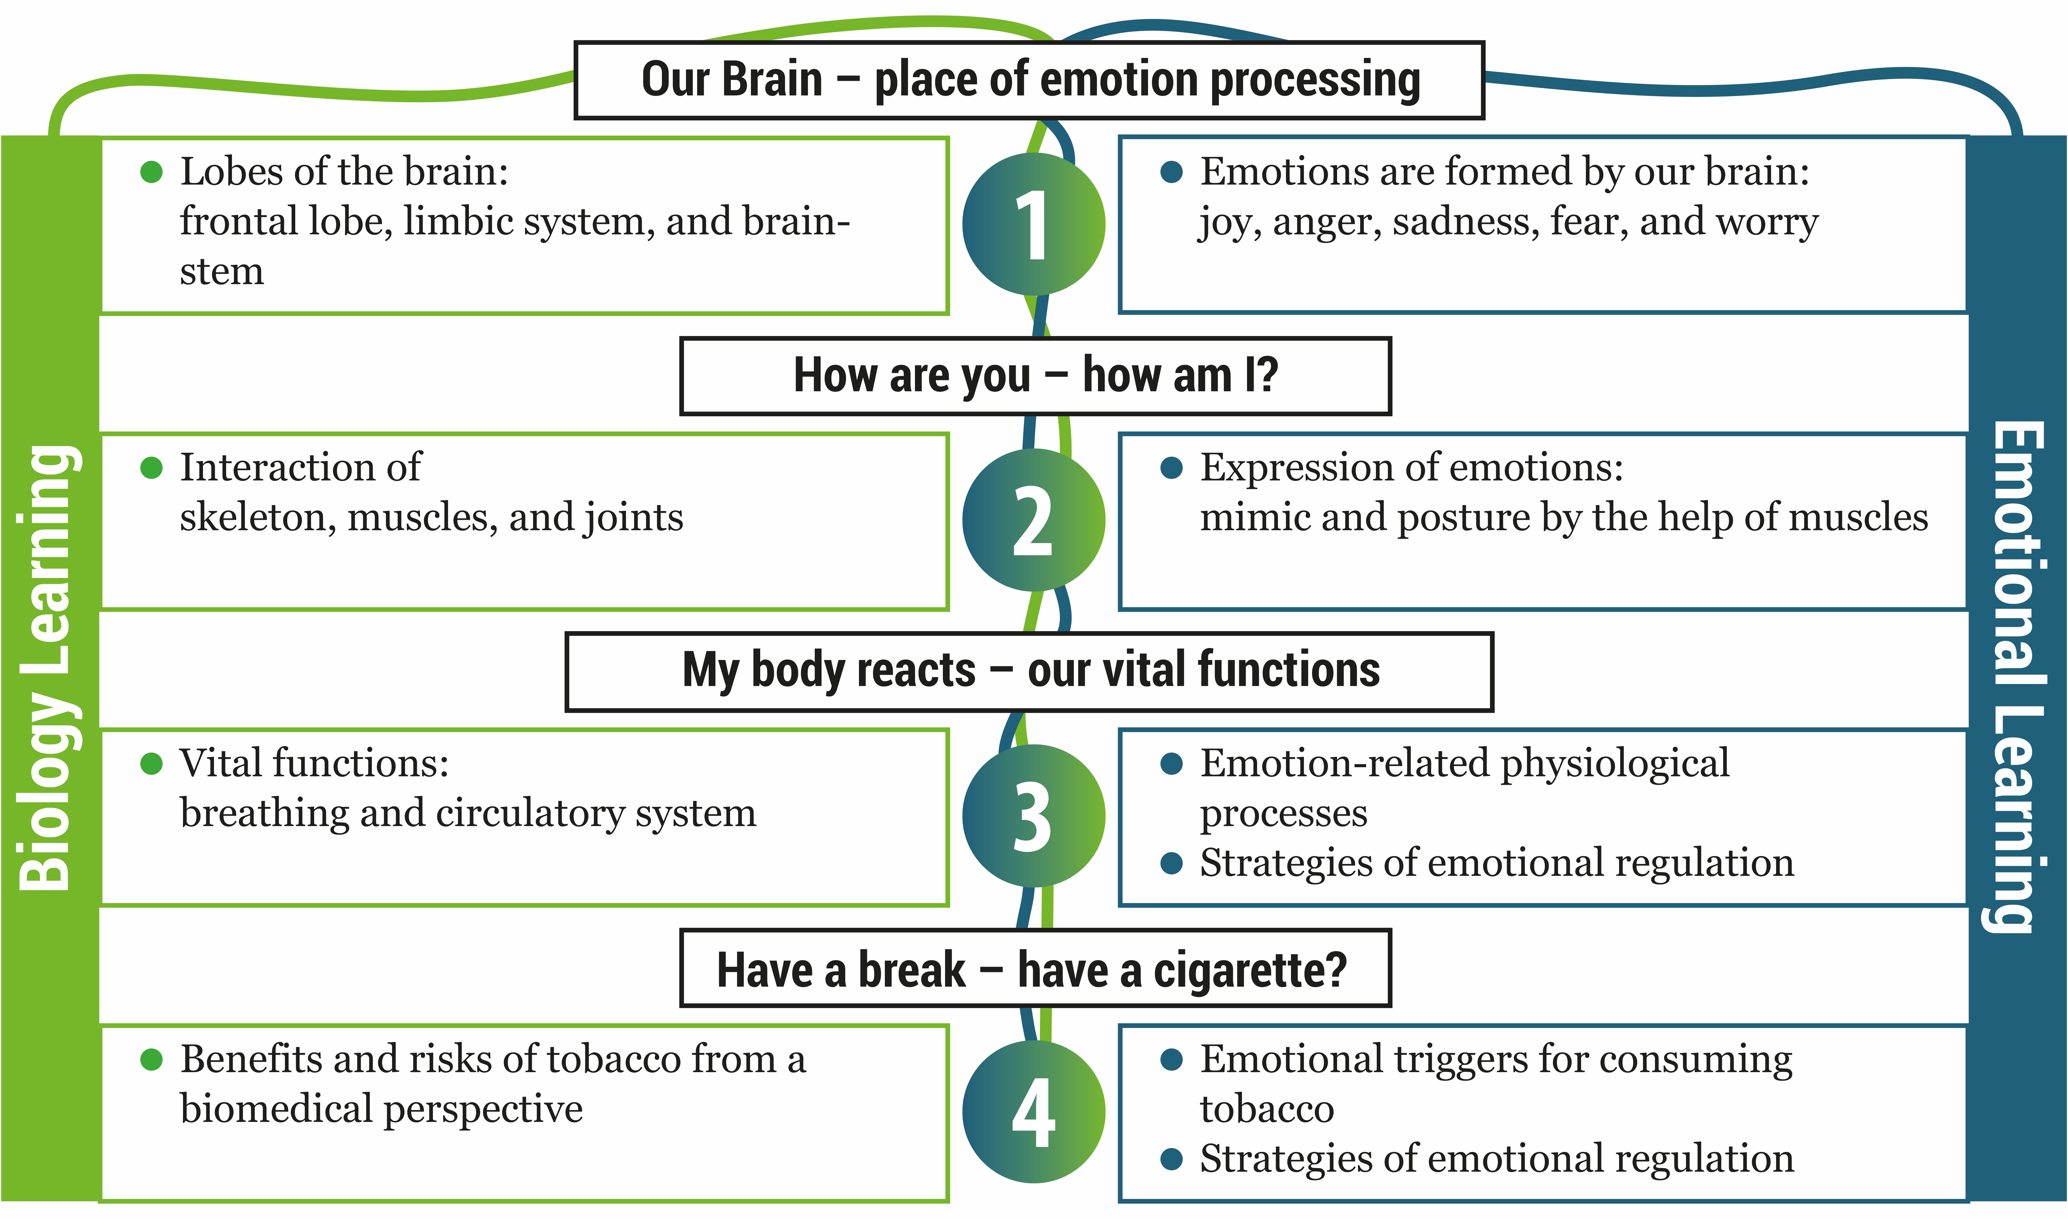
\includegraphics[width=1\textwidth]{images/fig1.png}
    \caption{Overview of the teaching units.}
\end{figure*}

Thus, each lesson covered both the physiological and psychological aspects. The relevant aspects of the human body were combined with corresponding aspects of emotional competence as part of SEL. These competences were derived from a model by Pons, Harris, and de Rosnay (2004) that describes a nine-step development of emotional competences:

\begin{enumerate}
    \item Recognition: To recognize and name emotions on the basis of expressive cues.
    \item External cause: To understand how external causes affect the emotions of others.
    \item Desire: Expectations are understood as emotional triggers.
    \item Belief - Emotional Perspective - ToM (Theory of Mind): Ability to understand the emotional perspective and feelings of others.
    \item Reminder: Understanding that stored memories can once again trigger emotions.
    \item Regulation: The ability to influence one’s own emotional state.
    \item Hiding Emotions: The ability to hide your own emotions.
    \item Mixed emotions: Understanding that you can have multiple emotions at the same time.
    \item Morality: Understanding of emotions that arise from the social context.
\end{enumerate}
(Pons et al., 2004)

The link between the listed emotional competences and the subject of the human body becomes clear in many ways. One good example is the way the human body reacts to anxiety (emotional competence 1): We open our eyes and mouth wide (somatic marker). Another example is the regulation of emotions (emotional competence 6): In an exciting situation, we can achieve physical calm by breathing deeply in and out. These are just two of the many examples used in the teaching series. Figure 1 gives an overview of how the human body, on the right-hand side, and emotional learning, on the left-hand side, were combined in the overall teaching series, and Figure 2 demonstrates this in the context of an individual lesson. 

\begin{figure*}[!h]
    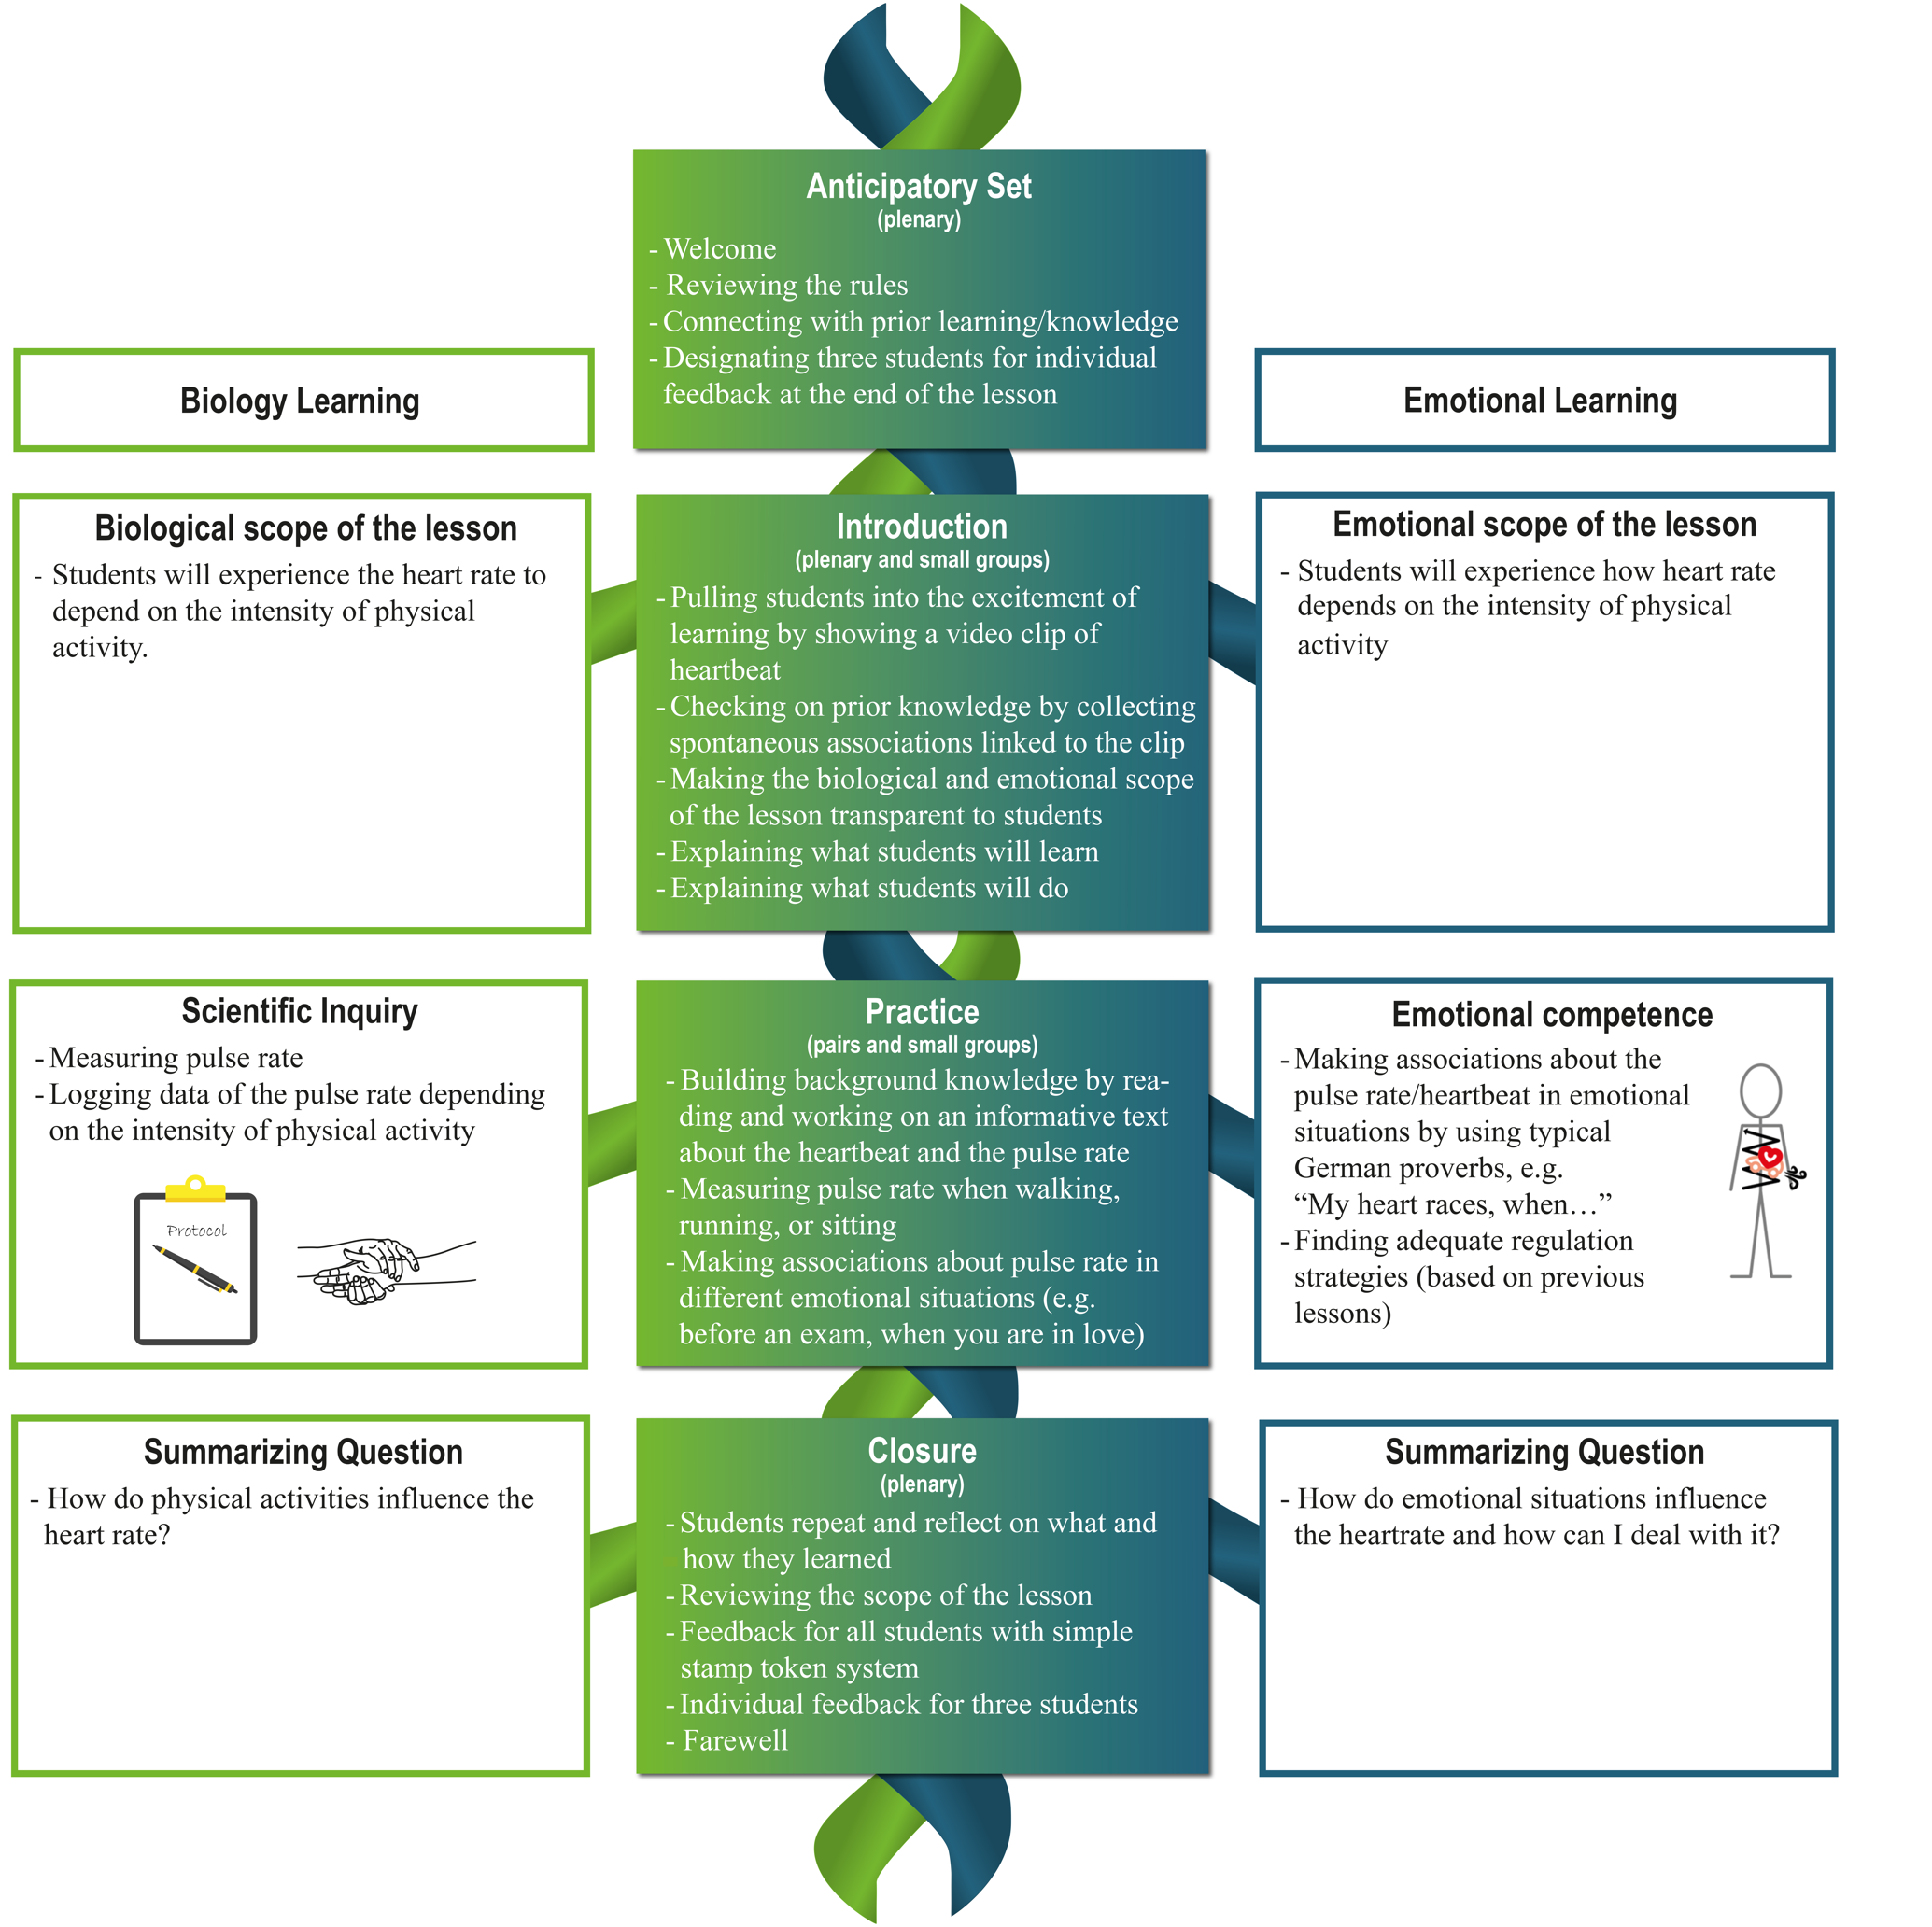
\includegraphics[width=1\textwidth]{images/fig2.png}
    \caption{Sample lesson}
\end{figure*}

To improve clarity and structure as important CM elements, the biological learning objectives and the SEL-related objectives were named and explained at the beginning of each lesson and recapitulated at the end. In order to allow for meaningful and cumulative learning, each lesson builds on the previous and uses active ways of learning.

Before the five teachers started to teach using the inclusive teaching approach, they took part in a 90-minute introductory course. In this introduction, the teachers received information about the CM strategies used in the lessons and various aspects of emotional competence in a brief presentation. Detailed examples were given and discussed in the context of the teaching series. Thereafter, the five teachers received the programmed teaching series plan, including instructions for every lesson as well as fully developed classroom materials. During this introduction, the teachers had the opportunity to peruse the plan and the materials and to ask questions. The introduction aimed to help the teachers conduct the teaching sequence in the way intended by the researchers/authors of this article. For the same purpose, a biology education student was assigned to each class and attended every lesson. These education students ensured easy communication between teachers and researchers, meeting with the researchers once a week to discuss teachers’ questions and report on the teachers’ success in following the lesson plan.

\begin{table*}[t]
\caption{Demographic Data}
\begin{tabular}{lcccc}
\hline
Teacher identification code & No. of classes taught by the teacher & Age (years) & Teaching experience (years) & Gender \\ \hline
01.01. & 3 & 46 & 9.5 & Male \\
01.04. & 3 & 49 & 10 & Male \\
02.01. & 1 & 30 & 4 & Male \\
02.02. & 1 & 52 & 20 & Female \\
03.01. & 1 & 24 & 2 & Female \\ \hline
\end{tabular}
\end{table*}

\subsection*{Database and Participants}

The sample consists of five secondary school teachers, three men and two women. Table 2 gives an overview of their demographic data. All teachers teach biology in grades five and six at four different public schools in and around the city of Cologne (Germany). The teachers were between 24 and 52 years old (\textit{M} = 40.2, \textit{Mdn} = 46) and had work experience ranging from 2 to 20 years (\textit{M} = 9.1, \textit{Mdn} = 9.5).

Guided interviews were used to collect data subsequent to the intervention. The interview questions covered seven different fields to gain a broad impression of teachers’ perception of the inclusive teaching approach: (a) experiences with the programmed teaching series plan, (b) implementation of CM, (c) pupils’ emotional development, (d) the perceived general effect on pupils (apart from their emotional development), (e) differences between the inclusive teaching approach and regular biology lessons, (f) changes in teachers’ attitude towards inclusion, and, finally (g) any further individual comments. 

\subsection*{Procedures}

The interviews took place after typical school hours in the schools where the teachers taught biology in the particular classes. All interviews were conducted by the first author and audio-taped. They then were transcribed and checked for accuracy. The transcripts were coded with MAXQDA 2018 (VERBI Software, 2017) for further analysis. The available data were examined with the help of qualitative content analysis (Hsieh \& Shannon, 2005; Schreier, 2012). As a first step, categories were derived deductively from the theoretical background described above. Hence, the categories were created for all elements of the intervention study, i.e. CM strategies, aspects of emotional competence, and biological content. In the second step, the category system was inductively expanded and partly restructured by two independent raters on the basis of the teachers’ answers. For this purpose, the raters analyzed part of interview material (approx. 20\%) based on the theoretically-derived category system. Based on their discussion about issues like imprecise descriptions, low discrimination, or missing categories, the system was expanded and restructured. In the third step, the first author and a second independent rater coded all of the data material using the final coding framework consisting of main categories (e.g. classroom management), sub categories (e.g. managing appropriate student behavior), definitions/explanations (e.g. using a token system in the form of a thumb punch for each lesson and student and giving individual feedback to selected learners in each lesson), leading questions (e.g. What do teachers report about the token system?), and typical examples (e.g. teacher 03.01: “I found the token system very good, because it was actually very simple. You [the teacher] had this stamp and did not have to argue for long whether you [the student] reached for the goal— yes or no. The students were able to confirm this [feedback] themselves: ‘Do I [the student] understand this or not?’”). A sufficient overall interrater reliability (Cohen’s kappa) of .91 was calculated using the standard procedure of MAXQDA (VERBI Software, 2017) following Brennan and Prediger (1981).

\section*{RESULTS}

To give an overview of the assigned codes, a distribution of their frequencies is listed in Table 3. We note that teaching preparation and CM were the most frequently represented topics the teachers talked about. In the following, one to three examples of the teachers’ responses are presented as original statements followed by a short summary of their main perceptions in each category. The quotations are assigned a teacher code at the end of each statement.

\begin{table}[ht]
\caption{The Category System and Total Number of Codings}
\begin{tabular}{lr}
\hline
Category & Number of Codings \\ \hline
General feedback & 87 \\
Appropriate lesson preparation and realization of the instructions & 247 \\
Different forms of implementation & 44 \\
CM & 219 \\
Intertwining of SEL and biology subject matters & 53 \\
Human body & 166 \\
Differences from regular/own biology lessons & 65 \\
Emotional competence & 148 \\ \hline
\end{tabular}
\end{table}

\subsection*{General Feedback}

\begin{quote}
    So overall, I’d say I got along well [with the teaching series]. Because there were different ways and possibilities to approach it, it was easy to introduce the children to a topic no matter in which form this happened. (01.04.)

    First of all, the intervention has been well accepted... (01.01.) My personal workload was now low, yet I was able to give good quality lessons with a lot of visual material. (02.02.)
\end{quote}

Overall, the teachers stated that they considered the use and implementation of the IBE teaching series a success and gave different reasons for this. Several teachers mentioned that they had less work to do because the project developers planned the lessons and provided the teaching material and media. In addition, some teachers reported that the quality of their teaching increased, as such a high-quality level is unlikely to be achieved in everyday school classes due to a lack of preparation time. They claim that the development of teaching materials and lessons for different levels of learning takes more time than is available due to other responsibilities, such as the evaluation of student tests or administrative work. In particular, the structure of the teaching series and the lessons, the activity-orientation, the variety of methods, and the differentiation of the materials for different levels of learning were viewed positively. 

\subsection*{Appropriate Teaching Preparation}

\begin{quote}
    Overall, I liked the lessons. Well structured, too. So, you knew how much time to plan for each task. (03.01.)
\end{quote}

According to their own statements, the teachers had worked with the IBE teaching series plan and used it in preparing their lessons. The plans and the contents were viewed as clearly developed and well organized. The implementation in the classroom involved no difficulties. At some points, teachers reported that they had implemented plans without themselves fully understanding their respective backgrounds, e.g. why a certain method was used or what the purpose of a particular task was. This lack of understanding could be remedied during the interviews. Therefore, it can be assumed that continual backing would have improved teachers’ understanding. Various planning elements were seen positively by some teachers and critically by others, e.g., open versus closed teaching situations (see CM below). Some teachers said that they dislike open learning situations because they are harder to manage, and thus the teachers felt more comfortable with closed teaching situations. In contrast, other teachers enjoyed the open learning environment because it allowed them to observe their pupils and their interactions.

\subsection*{Different Forms of Implementation}

\begin{quote}
    It was still a little bit so, that it disturbed me of course to stick to such a framework. If you’re used to planning your lessons yourself and adapting them to a group, then it’s always a bit like “Oh no! It's different now and I have to do it this way,” although I would have had a different idea at that point. So that was difficult for me until the very last moment. (02.02.)
\end{quote}

The teachers reported that in terms of lesson preparation, it was new to them to teach a lesson that had been prepared by someone else. They first had to understand the lessons themselves before they could teach them. The opinions of how challenging this was varied; thus, one reported that she had to suppress her impulse to follow her own ideas rather than those provided by the plan at the very beginning. Other mentioned that they simply did what was explained in the plan, sometimes without realizing what they were doing in detail. Some teachers modified the plan according to their needs, e.g., because they were short of time. Small modifications, like skipping optional tasks, had no impact on our results. Two classes were excluded before the final analyses because their accompanying graduate students reported significant deviations from the plan. To the best of our knowledge, in all other classes teachers essentially followed the lesson plan.

\subsection*{Teaching Material}

\begin{quote}
    I found the material absolutely versatile. The workbooks [were] well thought out. (02.02.)
    
    It was good for our pupils with special needs that they always had an overview of what was coming up next. (02.01.)
\end{quote}

The feedback about the materials was very positive. The workbooks provided were seen as a good alternative to books and loose worksheet papers. They particularly liked the design, which they considered pupil-friendly and age appropriate. The teachers also reported that the pupils gave them positive feedback about the workbooks. However, as we did not collect further data about pupils’ perceptions, detailed explanations must be further investigated. The workbooks were adjusted to different levels of knowledge and competencies according to the diverse prerequisites of the pupils, and teachers were advised to administer them accordingly. The teachers admitted that these adjusted workbooks were somehow required, but their acceptance by pupils differed from class to class. While some pupils, even good ones, preferred to work with the easiest workbook, others, including some of the students with learning difficulties, preferred to work with more complex ones. The teachers also chose different ways of assigning the workbooks: Some let the pupils choose them themselves while others decided for their pupils. The other materials (e.g., posters and pictures) were also mentioned frequently in the interviews. The teachers liked them, as they could use them in many ways during the lessons.

\subsection*{Methods}

\begin{quote}
    The variety of methods was great for both the pupils and me. (01.01.)
\end{quote}

The teachers explained that the variety of methods had a positive effect on their teaching. They observed that the pupils were motivated and showed a high level of active involvement and participation. For some methods (e.g., role playing, model making), no general agreement was found as to whether they were suitable for the pupils and the extent to which they should be introduced. Various models (e.g., papier-mâché brain models, vertebrae made of salt dough), experiments (e.g., pressure on tubular and flat bones, measurement of lung volume), and a practical examination (dissection of a lamb heart) were used. The teachers perceived these scientific working methods differently. Some criticized the assembly of a joint model for being too simple. The majority, however, reacted positively. Several teachers said that they plan to pay more attention to greater methodological diversity in the future and that they want to make their own teaching more action-oriented.

\subsection*{Classroom Management}

\begin{quote}
    I know we talked about these three rules at the beginning, but that was it. (02.02.)
\end{quote}

Three rules were introduced at the beginning of the series: (a) I am friendly, (b) I raise my hand when I want to say something, and (c) I am quiet and I listen. One teacher remarked that a more intensive introduction would be necessary and that the rules should be repeated at the beginning and end of each lesson. Another teacher explained that they were self-evident and therefore did not require any kind of introduction.

\begin{quote}
    I have noticed that it was always clear what was going to happen next.
    
    The objectives of each lesson were pointed out clearly. (03.01)
\end{quote}

The clarity of the teaching, which was promoted in the teaching unit by citing the objectives of the lessons and providing transparency regarding the course of the lessons, was particularly emphasized by several teachers. They explained that this clarity provided good guidance to the pupils.

\begin{quote}
    At the end of a lesson, you see [the result]: how did I behave as a student? You [as a student] get feedback, which allows you to think about yourself again. (02.01)
\end{quote}

A token system was introduced for positive feedback. The majority of the teachers viewed this system positively and reported that individual feedback given to three previously selected pupils per lesson had positive effects because all the pupils made more effort. They also appreciated the easy handling of the token system, as each pupil simply received a stamp at the end of the lesson. A positive effect from the teachers’ perspective was that pupils did not stay after the lesson to ask about their performance, because the token system provided sufficient feedback.

\begin{quote}
    There were a few things where it got too noisy for me. So, sometimes the classes could manage running from A to B to C quite well. (01.04.)
\end{quote}

Regarding the teacher-centered and open teaching elements in the lessons, three teachers said that as disturbances occurred in the open teaching situations, they would prefer teacher-centered lessons.

\subsection*{Intertwining of SEL and Biology Subject Matters}

\begin{quote}
    I found the intertwining [of biological and SEL content] within the series very, very close. Both were repeatedly pointed out. (03.01.)
    
    Transparent to me was the field where we talked about emotions [and how these are] linked to the brain: Where do they happen, what blocks [them]? The children understood this, too. (02.01.)
\end{quote}

The intertwining of biological subject matter and SEL within the approach was not fully perceived by all teachers. Only one teacher noticed that both fields were continuously woven together. Others identified core topics, especially at the beginning of the teaching series. Almost all teachers understood how the human brain (brain stem, limbic system and prefrontal cortex) and basic emotions are connected. It was also clear to them how emotions affect facial expressions, mimetic muscles, posture, skeleton, musculature, and joints. In contrast, not all of them were aware of the connection between vital functions and regulation of emotions.

\begin{quote}
    I hadn’t been aware of that until now. My God, how nice to talk to you about this again. (01.01.)
\end{quote}

However, one teacher only just realized in the interview that there were connections between SEL and biology subject matters. Interestingly, he concluded that his pupils seemed to be aware of the connections even though he had not pointed them out explicitly. Admittedly, the interviews do not provide sufficient data to draw a firm conclusion about this matter. However, it becomes obvious that teachers’ understanding of the connection decreased throughout the course of the study. Possible explanations might be that teachers thought about the theoretical concept of the teaching unit more thoroughly and prepared their lessons more conscientiously at the beginning of the intervention due to the recentness of the introduction and their unfamiliarity with the materials.

\subsection*{Human Biology Subject Matters}

\begin{quote}
    In any case, they learned a lot of biology (01.01.)
    
    At the end of the day, the bottom line is that for a specialist or natural scientist, everything was too little. Little has been transported. Everything has just been scratched. (01.04.)
\end{quote}

The teachers viewed the learning success with regard to biology subject matters differently. Some said that the pupils had learned a lot in terms of the subject, but also that too little content was taught. Only a knowledge test could provide reliable information. However, the teachers agreed that the interest of the pupils in the subject matter had been awakened. Some teachers said that one cannot expect more because the teaching series was restricted to only two hours per week.
There were obvious differences in how often certain topics were recalled by the teachers in the interviews (see Table 3). Teachers mainly talked about the skeleton, the musculature, the joints, and the vital functions. The topics of the lobes of the brain and risks of tobacco from a biomedical perspective were hardly discussed by the teachers. A reason for this might be that these last two topics are not necessarily part of the curriculum for fifth- and sixth-graders but are usually taught in older classes. In terms of teaching methods, they mainly mentioned the experiments, the models, and the practical examination (i.e., dissection of the heart). These were the more elaborate elements of teaching which required more extensive preparation by the teachers and, therefore, might be used less frequently in class and be more impressive for them.

\subsection*{Different from Regular Biology Classes}

\begin{quote}
    In the regular biology lessons, you often orient yourself toward the book you have in school. And now with the series, it was such that we also included current things, like a movie, for example. The students found this extremely motivating. (03.01.)
    
    That was a teaching series, [...], that’s not so stringent for me. But I have the feeling that the pupils liked it that way. (01.01.)
\end{quote}

Unlike their self-prepared biology lessons, the teachers explained that the teaching series was not based on a biology book. Instead, it made use of current materials and media (e.g., film excerpts). The teachers did not use the token system in regular biology lessons either, because they did not consider it their responsibility to reward their pupils. Some teachers explained that the teaching series made it possible to focus on a particular subject field, which was an advantage. Furthermore, some teachers admitted that they generally do not prepare their lessons adapted to the diversity of pupils’ individual needs because this would require excessive time. As a consequence, when preparing their lessons, they predominantly kept the pupils with learning difficulties in mind. This lack of adaptivity is obviously in conflict with the UN convention and other guidelines, but it seems to be fairly common in practice and might indicate the excessive demands placed on teachers. One teacher explained that she has learned through the teaching series that there are ways to teach even complex topics (i.e., the brain) in inclusive classes. This, however, requires that the material be prepared adequately.

\subsection*{Emotional Competence}

\begin{quote}
    But I believe that the naming of these [emotions] has already raised a different awareness among the children. (01.04.)
\end{quote}

From the teachers’ point of view, there was a significant increase in emotional competences, especially in the recognition and naming of emotions. The pupils were now able to recognize more quickly and more precisely from facial expression and body posture how their classmates felt.

\begin{quote}
    I would say there has been a little development. Especially when it came to someone who didn’t feel well. Now, it was less that he [the other student] annoyed me, but rather that he [the other student] wasn’t doing well. (01.04.)
\end{quote}

The pupils were also able to realize in which situation their fellow pupils were, take this into account, and respect their emotional states.

\begin{quote}
    As I said, as far as regulation [of emotions] is concerned, I do not know whether the two hours or one hour a week is enough to really help the students regulate themselves. I do know they loved the relaxation exercises and they thought it was good for them. (03.01.)
\end{quote}

The teachers mentioned the field of emotional self-regulation in which the pupils focused on the perception of their own emotions and the associated effects. They assumed that a long-term change in terms of emotion self-regulation would require more intensive training. However, this training could not be realized within the two hours of biology lessons per week. In this context, it is also interesting that they found it difficult to make a more precise assessment of how the emotional competences of their pupils developed. They argued that they spent too little time with their pupils to be able to evaluate the development of emotional regulation in particular. The issue with the assessment of emotional regulation seems to be that it is difficult to observe concretely. In contrast, teachers found it easier to evaluate students’ development regarding recognition of emotions because it can be observed directly in the lessons when miming or decoding facial expression on photographs, for example. 

\subsection*{Impact on Pupils}

\begin{quote}
    There is one [pupil], I know that at the beginning he was very challenging in his behavior, because he was very loud, very disruptive. This has been extremely dialed back. And then there was one who at the beginning had very, very strong problems with starting tasks, having his things with him, working when the working phases took place, working with partners, participating. And that has been extremely changed in the last few weeks. I have never seen a child change so quickly. (03.01.)
\end{quote}

Several teachers reported that they have noticed significant changes in some pupils’ behavior. For example, two pupils with challenging behavior started to behave better. However, teachers were unable to give a causal explanation for this. Teachers noticed improvements in terms of the learning and working behavior of some pupils as well. These pupils now had their working materials with them and were willing to participate and cooperate in the working phases. One teacher also said that their more introverted pupils dared to present things to the class in the teaching series’ role-plays.

Furthermore, several teachers explained that because emotions are such a personal topic, they could gain closer access to their pupils. They were able to speak about emotions with the class and this helped the rather shy pupils to get in touch with their teachers. This closer contact then allowed the pupils to share what they thought about their personal learning success, not only in biology but also in other subjects.

\subsection*{Impact on Teachers}

The teachers said that teaching following this approach has raised their awareness of the importance of teaching in a more socio-emotional way, which was new to them. One was encouraged to include SEL elements in her lessons in the future, and stated that she will particularly pay more attention to SEL in her lower secondary school classes. According to her, SEL is indeed a prerequisite for higher secondary school education, as the focus then is more on subject-matter topics.

Another teacher argued that because of the clear combination of human biological subject matters (in this case the brain) and the associated emotional competences, it is now easier to see which learning disorders may occur. The majority of the teachers stated that they intend to use a broader methodological repertoire in the future. For example, they are planning to use cooperative learning situations, digital devices, and media such as films more often in their lessons. Furthermore, they explained that they will pay more attention to the performance and learning success of all pupils.

\section*{DISCUSSION, IMPLICATIONS, AND OUT\-LOOK}

Overall, the teachers’ interviews give a positive picture of the IBE approach. Regarding the core elements (human body, emotional learning, and CM), teachers’ perceptions are versatile. On the whole, teachers perceive them as valuable and fruitful in general, but there is some critique of the particular realization. Interestingly, some teachers did not realize the integration of SEL- and CM-centered elements in the teaching unit at all.

\section*{Learning about the Human Body}

To support pupils’ learning in biology class about the human body, we provided a broad spectrum of methods (e.g., the dissection of a heart, role-play) and graded workbooks in our approach. The intention was to motivate even pupils with EBD and to allow all pupils to learn biology regardless of their individual prior knowledge and prerequisites (cf. Scruggs \& Mastropieri, 2000). With this approach we followed the significance of individual prior knowledge for future learning (cf. Dochy, Segers, \& Buehl, 1999). The teachers often referred to these versatile methods in the interviews and promised to expand their methodological repertoire and make their teaching more action-oriented. This shows that these elements of our approach may impact biology teachers’ future teaching. The variety of the partly new methods and the positive experience in their own teaching seem to be important to this decision. This is not surprising as observing success is important for changing teachers’ teaching and beliefs (Haney, Czerniak, \& Lumpe, 1996). The matter of whether the teachers will actually change their teaching practice cannot be answered right now.

The workbooks were of particular interest to the teachers as well. Teachers reported disagreement over how to assign the graded workbooks to the pupils according to their prior knowledge and prerequisites. On the other hand, the advantages of the graded material became apparent very easily and the material was seen as beneficial, if not utterly necessary. Thanks to the grading of the workbooks, all pupils had the chance to experience a sense of achievement. This increased pupils’ motivation significantly.

Surprisingly, some teachers considered themselves unable to determine pupils’ learning success, as this would require a written test. This is somehow contradictory to their practice, as they assess pupils’ learning in their regular lessons. They seemed to be unaware of the differences between summative and formative assessment (cf. Black, 1993). This leads to the general question for the future of how learning assessments in inclusive biology classes will look, considering the very different starting points of the pupils.

\subsection*{Emotional Learning}

With regard to the emotional learning of their pupils, the teachers primarily referred to basic competences, such as recognizing emotions in themselves and others (Pons et al., 2004). Interestingly, while SEL was part of the entire teaching series, the teachers mainly referred to the first part of the intervention when considering the social-emotional development of their pupils. This might be because the teachers had become used to this element of the approach. However, it still seems unclear to individual teachers what emotional regulation in oneself and in others really means. A reason for this might be that teachers do not see the relevance of the theoretical background of such measures as described by Nash, Schlösser, and Scarr (2016). This lack of understanding of emotional regulation is consistent with our quantitative findings, which show an increase in pupils’ emotional competences in the following fields (cf. Rindermann, 2009): (a) recognition and understanding of their own emotions, (b) recognition of emotions in others, (c) assisting others to regulate their emotions, and (d) attitude toward emotions (Ferreira González, Hövel, Schlüter, Hennemann, \& Osipov, 2019). However, there was no detectable increase in pupils’ emotional self-regulation. These abilities of regulating one’s own emotions or replacing maladaptive strategies with adaptive strategies is particularly relevant at their age (Berk \& Meyers, 2015; Hughes et al., 2013; Salisch \& Vogelgesang, 2005), but teaching emotional competences successfully requires teachers to be aware of it (Nash et al., 2016). Thus, it is not surprising that we did not find changes in this regard, as the teachers were not really aware of this issue. A model to support teachers’ professional development in this regard could be existing training programs for parents that are adapted for teachers’ needs (M. T. Greenberg et al., 2017; Zinsser, Denham, Curby, \& Shewark, 2015). Several teachers said that their regular weekly biology class time of 90 to 120 minutes allow too little contact with the pupils to teach emotional regulation strategies effectively. This is a crucial situation as school is one of the most important places for students in middle childhood to meet adults supporting their positive development (Oberle, Schonert-Reichl, Guhn, Zumbo, \& Hertzman, 2014). This seems to be an important challenge, as the success of an inclusive school system requires a secure environment and relies on teachers who are able to build sustainable relationships with their students (Cornelius-White, 2007; Reicher, 2010). This raises the further question of how teachers’ awareness can be trained and how they can provide such an environment even if they teach a class only a few hours a week.

\subsection*{Classroom Management}

The teachers’ main positive feedback concerned the high quality of the teaching approach, especially the well-structured lessons and the teaching materials, which they liked for two main reasons: First, they had the impression of a high-quality teaching compared to their own regular lessons, and, second, they appreciated the reduction of their personal workload by the teaching series and materials provided. Thus, all in all, the teachers had a largely positive experience with this approach, including a perceived increase of general teaching quality. These findings show once again the crucial role that the preparation of lessons plays in teaching quality (cf. Hattie, 2012) and raises further questions for future research: To what extent do teachers have enough time and resources in their everyday practice to provide high-quality teaching? To what extent could already prepared teaching materials be supportive? To what extent could a professional development program with examples of good teaching qualify teachers to prepare and conduct intertwined SEL and biology lessons themselves? 

All in all, it was obvious that the teachers did not notice all the integrated elements of CM (Emmer \& Evertson, 2013; Emmer \& Sabornie, 2015). This raises the question whether the teachers were so familiar with the CM that they did not wish to talk about these strategies or instead needed professional development (cf. Herzmann \& König, 2016). In this regard participants’ teaching experience might be an important factor because there are differences regarding CM use of expert and novice teachers. Some of the teachers seemed to be insecure with open teaching situations and reported that they felt more comfortable with direct instruction. Interestingly, they assumed that direct instruction was more effective for learning, which is true for students with learning disabilities (Archer \& Hughes, 2010).

\section*{CONCLUSION}

Based on the teachers’ feedback, one can assume that detailed lesson plans and good, easy to handle teaching materials could be a useful tool to implement inclusive teaching practice in everyday school (cf. Thompson \& Zeuli, 1999), but this is not without limitations. Thus, the teachers often emphasized that the clearly defined series plans gave more structure to their own teaching. However, they stated that they also lost some of their personal flexibility due to the lesson plan. This individual flexibility seems to be very important, because the teachers’ preferences vary regarding the application of the workbooks, particular methods (e.g., role-play), introduction of rules, and teaching situations (open vs. closed). Hence, for a lesson plan and learning materials to be successfully implemented in school, they should address the core ideas (e.g., of inclusive teaching) but not override the teachers, instead allowing every teacher to follow his or her own teaching style and make learning suitable for all the pupils in science class. This is consistent with other findings, e. g. that “teachers wanted SEL curricula for their classroom, but they did not want a scripted curricula” (Humphries et al., 2018, p. 168).

To conclude, an elaborated teaching sequence with manifold materials and methods can facilitate the implementation of inclusive teaching in everyday school, but there is no universal solution suitable for every purpose. The “simple things” in particular seem to be suited to implementation, like the token system and the portfolio of methods. In conclusion, it seems possible to implement a dual teaching approach bringing together biology and SE learning in everyday school.

\section*{LIMITATIONS}

The interview guide used during the interviews ensured that all relevant aspects included in the learning approach (human body, SEL, CM) were considered. During the coding and summary of the interviews, it became clear that the teachers often only focused on specific—mainly practical—elements of the teaching series and that a perspective on the overall picture is missing in many cases. A reason for this could be the long time of the intervention itself, with one interview at the end. An alternative procedure would have been to conduct several interviews during the course of the intervention, such as after each section of the series, but this could have been a kind of additional intervention, which was not intended. For further research one might consider more frequent meetings between the researchers and teachers to facilitate the teachers in their development and implementation as duration of activity is a significant structural feature in professional development (Garet, Porter, Desimone, Birman, \& Yoon, 2001).

This study provides evidence that teachers see the use and implementation of SEL in inclusive biology lessons as a valuable enrichment for all pupils. This added value was reported by the teachers, both for themselves and for pupils. However, further implementation measures seem necessary. A 90-minute introduction and programmed material are not enough to teach teachers the basics and contents of the teaching series. This raises the question of the extent to which further training and support for teachers is feasible. A possibility would be to expand the introduction for the teachers and to subdivide it into more “handy” parts. Teachers could implement the introduced concepts and lessons into their teaching practice one at a time. Also, by reflecting on their experiences with the researchers, they could extract the core ideas of SEL and could subsequently apply these core ideas to their own lesson planning and teaching material development, continuously supported by researchers or trainers. 

The IBE series only covers a subset of social and emotional competence and a single subject, biology. Whether this teaching concept would also succeed for other content fields must be clarified in further investigations, especially as our biological topic of the human body seems ideal for intertwining with SEL. Finally, our study could not provide evidence for the efficacy of any particular CM strategy (e.g. the token system), as we used a bundle of measures to show their compatibility with other measures (biology learning, SEL). More detailed analyses will require research designs with isolated strategies.

\subsection*{ACKNOWLEDGEMENTS}

The authors would like to express their gratitude to all teachers and students for their participation, particularly to Daria Eichhöfer, Bastian Geschwind, and Sarah Ricke for their great efforts. They would also like to thank Benjamin Salomon and Elisabeth Helmrath for their support as independent raters.


\end{large}
\clearpage
\section*{REFERENCES}\par 

\leftskip 0.25in
\parindent -0.25in 
Akelaitis, A. V., \& Lisinskiene, A. R. (2018). Social emotional skills and prosocial behaviour among 15–16-year-old adolescents. \textit{European Journal of Contemporary Education, 7}(1), 21–28. doi:10.13187/ejced.2018.1.21

Arbeiter, S. \& Hartley, S. (2002). Teachers´and Pupils´ Experiences of Integrated Education in Uganda. \textit{International Journal of Disability, Development and Education, 49}(1), 61-78. doi:10.1080/10349120120115334

Archer, A. L., \& Hughes, C. A. (2010). \textit{Explicit Instruction: Effective and Efficient Teaching}. New York: Guilford.

Berk, L. E., \& Meyers, A. (2015). \textit{Infants, children, and adolescents} (8th ed.). Boston: Pearson.

Black, P. J. (1993) Formative and summative assessment by teachers. \textit{Studies in Science Education, 21}(1), 49-97. doi:10.1080/03057269308560014

Brennan, R. L. and D. J. Prediger (1981). "Coefficient Kappa: Some uses, misuses, and alternatives." \textit{Educational and Psychological Measurement, 41}(3): 687-699. doi:10.1177/001316448104100307

Buchanan, R., Gueldner, B. A., Tran, O. K., \& Merrell, K. W. (2009). Social and emotional learning in classrooms: A survey of teachers’ knowledge, perceptions, and practices. \textit{Journal of Applied School Psychology, 25}(2), 187–203. doi:10.1080/15377900802487078

CASEL/Collaborative for Academic, Social, and Emotional Learning. (2017). What is SEL. Retrieved from \url{https://casel.org/what-is-sel/}

Conderman, G. (2011). Middle school co-teaching: Effective pracitices and student reflections. \textit{Middle School Journal, 42}(9), 24–31.

Cornelius-White, J. (2007). Learner-centered teacher-student relationships are effective: A meta-analysis. \textit{Review of Educational Research, 77}(1), 113–143. doi:10.3102/0034-65430298563

Dochy, F. R. C., Segers, M., \& Buehl, M. M. (1999). The relation between assessment practices and outcomes of Studies: The case of research on prior knowledge. \textit{Review of Educational Research, 69}(2), 145–186. doi:10.3102/003\-46543069002145

Durlak, J. A., Weissberg, R. P., Dymnicki, A. B., Taylor, R. D., \& Schellinger, K. B. (2011). The impact of enhancing students’ social and emotional learning: A meta-analysis of school-based universal interventions. \textit{Child Development, 82}(1), 405–432. doi:10.1111/j.1467-8624.2010.01564.x

Elias, M. J., Zins, J. E., Weissberg, R. P., Frey, K. S., Greenberg, M. T., Haynes, N. M., . . . Shriver, T. P. (1997). \textit{Promoting social and emotional learning: Guidelines for educators}. Alexandria: ASCD.

Emmer, E. T. \& Evertson, C. M. (2013). Classroom Management for Middle and High School Teachers (9th ed.). Upper Saddle River, NJ: Pearson.

Emmer, E. T. \& Sabornie, E. J. (2015). Handbook of Classroom Management (2nd ed.). New York: Routledge.

Evertson, C. M., \& Weinstein, C. S. (2006). Classroom management as a field of inquiry. In C. M. Evertson \& C. S. Weinstein (Eds.), \textit{Handbook of classroom management: Research, practice, and contemporary issues} (pp. 3–15). New York: Routledge.

Ferreira González, L., Hövel, D. C., Schlüter, K., Hennemann, T., \& Osipov, I. (under review). Emotionale Kompetenzförderung im inklusiven Biounterricht. [Promotion emotional competence in inclusive biology lessons]. \textit{Prävention und Gesundheitsförderung}.

Ferreira González, L., Leidig, T., Hennemann, T., \& Schlüter, K. (2016). IBU - Inklusiver Biologieunterricht [IBE - Inclusive Biology Education]. In J. Menthe, D. Höttecke, T. Zabka, M. Hammann, \& M. Rothgangel (Eds.), \textit{Befähigung zu gesellschaftlicher Teilhabe. Beiträge der fachdidaktischen Forschung} [\textit{Empowerment to participate in society: Contributions of educational research}] (Vol. 10, pp. 335–350). Münster: Waxmann.

Forlin, C., Keen, M., \& Barrett, E. (2008). The concerns of mainstream teachers: Coping with inclusivity in an Australian context. \textit{International Journal of Disability Development and Education, 55}(3), 251–264. doi:10.1080/\-10349120802268396

Garet, M. S., Porter, A. C., Desimone, L., Birman, B., \& Suk Yoon, K. (2001). What makes professional development effective? Results from a national sample of teachers. \textit{American Educational Research Journal, 38}(4), 915-945. doi:10.3102/00028312038004915

Georgi, V. B. (2015). Integration, Diversity, Inklusion: Anmerkungen zu aktuellen Debatten in der deutschen Migrationsgesellschaft. [Integration, diversity, inclusion: Comments on current debates in the German migration society.] \textit{Die Zeitschrift für Erwachsenenbildung 2015}(02), 25–27.

Gidlund, U., \& Boström, L. (2017). What is inclusive didactics? Teachers’ understanding of inclusive didactics for students with EBD in Swedish mainstream school. \textit{International Education Studies, 10}(5), 87–99. doi:10.5539/\-ies.v10n5p87

Greenberg, J., Putman, H., \& Walsh, K. (2014). Training our future teachers: Classroom management (2nd ed.). Washington: National Council on Teacher Quality. Retrieved from \url{https://www.nctq.org/dmsView/Future_Teachers_Classroom_Management_NCTQ_Report}

Greenberg, M. T., Domitrovich, C., Weissberg, R. P., \& Durlak, J. A. (2017). Social and emotional learning as a public health approach to education. \textit{The Future of Children, 27}(1), 13–32.

Greenberg, M. T., Weissberg, R. P., O´Brien, M. T., Zins, J. E., Fredericks, I., Resnik, H., \& Elias, M. J. (2003). Enhancing school-based prevention and youth development through coordinated social, emotional, and academic learning. \textit{American Psychologist, 58}, 466–474. doi:10.1037/0003-066X.58.6-7.466

Haney, J. J., Czerniak, C. M., \& Lumpe, A. T. (1996). Teacher beliefs and intentions regarding the implemantation of science education reform strands. Journal of Research in Science Teaching, 33, 971-993. doi:10.1002/\-(SICI)1098-2736(199611)33:9<971::AID-TEA2>3.0.CO;2-S

Hattie, J. (2012). \textit{Visible learning for teachers. Maximizing impact on learning}. London: Routledge.

Helmke, A., \& Helmke, T. (2015). Wie wirksam ist gute Klassenführung? Effiziente Klassenführung ist nicht alles, aber ohne sie geht alles andere gar nicht. [How effective is good classroom management? Efficient classroom management is not everything, but without it everything else does not work at all.] \textit{Pädagogik Leben, 2}, 7–11.

Herzmann, P. \& König, J. (2016). \textit{Lehrerberuf und Lehrerbildung}. [\textit{Teaching profession and teacher training}.] Bad Heilbrunn: Klinkhardt.

Hsieh, H.-F., \& Shannon, S. E. (2005). Three approaches to qualitative content analysis. \textit{Qualitative Health Research, 15}(9), 1277–1288. doi:10.1177/1049732305276687

Hughes, L. A., Banks, P., \& Terras, M. M. (2013). Secondary school transition for children with special educational needs: A literature review. \textit{Support for Learning, 28}(1), 24–34. doi:10.1111/1467-9604.12012

Humphries, M. L., Williams, B. V., \& May, T. (2018). Early childhood teachers’ perspectives on social-emotional competence and learning in urban classrooms. \textit{Journal of Applied School Psychology, 34}(2), 157–179. doi:10.10\-80/15377903.2018.1425790

Hutchings, J., Martin-Forbes, P. A., Daley, D., \& Williams, M. E. (2013). A randomized controlled trial of the impact of a teacher classroom management program on the classroom behavior of children with and without behavior problems. \textit{Journal of School Psychology, 51}(5), 571–585. doi:10.1016/j.jsp.2013.08.001

Jennings, P. A., \& Greenberg, M. T. (2009). The prosocial classroom: Teacher social and emotional competence in relation to student and classroom outcomes. \textit{Review of Educational Research, 79}(1), 491–525. doi:10.3102/003\-4654308325693

Klassen, R. M., \& Anderson, C. J. K. (2009). How times change: Secondary teachers’ job satisfaction and dissatisfaction in 1962 and 2007. \textit{British Educational Research Journal, 35}(5), 745–759. doi:10.1080/01411920\-802688721

Korpershoek, H., Harms, T., de Boer, H., van Kuijk, M., \& Doolaard, S. (2016). A meta-analysis of the effects of classroom management strategies and classroom management programs on student’s academic, behavioral, emotional, and motivational outcomes. \textit{Review of Educational Research, 86}(3), 643–680. doi:10.3102/00346543\-15626799

Kyriacou, C. (2009). \textit{Effective Teaching Skills: Theory and Practice} (3rd ed.). Cheltenham: Nelton Thornes.

Lamport, M. A., Graves, L., \& Ward, A. (2012). Special needs students in inclusive classrooms: The impact of social interaction on educational outcomes for learners with emotional and behavioral disabilities. \textit{European Journal of Buisness and Social Sciences, 1}(5), 54–69. 

Martin, A. J., Linfoot, K., \& Stephenson, J. (1999). How teachers respond to concerns about misbehavior in their classroom. \textit{Psychology in the Schools, 36}(4), 347–358. doi:10.1002/(SICI)1520-6807(199907)36:4<347::AID-PIT\\S7>3.0.CO;2-G

MSW NRW / Ministerium für Schule und Weiterbildung des Landes Nordrhein-Westfalen (2013). \textit{Kernlehrplan für die Gesamtschulen- Sekundarstufe I in Nordrhein-Westfalen, Naturwissenschaften Biologie, Chemie, Physik}. [\textit{Core Curriculum for the Secondary School Level I in North Rhine-Westphalia, Natural Sciences Biology, Chemistry, Physics}]. Frechen: Ritterbach.

MSW NRW/Ministerium für Schule und Bildung des Landes Nordrhein-Westfalen (2018). Statistik-Telegramm 2017/18. Statistische Übersicht Nr. 397. [Statistics telegram 2017/18. Statistical Overview No. 397.] Retrieved from \url{https://www.schulministerium.nrw.de/docs/bp/Ministerium/Service/Schulstatistik/Amtliche-Schuldaten/StatTelegramm2017.pdf}

Nash, P., Schlösser, A. \& Scarr, T. (2016). Teachers’ perceptions of disruptive behaviour in schools: a psychological perspective. \textit{Emotional and Behavioural Difficulties, 21}(2), 167-180. doi:10.1080/13632752.2015.1054670

Oberle, E. (2018). Social-emotional competence and early adolescents’ peer acceptance in school: Examining the role of afternoon cortisol. \textit{PLoS One, 13}(2). doi:10.1371/\-journal.pone.0192639

Oberle, E., Schonert-Reichl, K. A., Guhn, M., Zumbo, B. D., \& Hertzman, C. (2014). The role of supportive adults in promoting positive development in middle childhood: a population-based study. \textit{Canadian Journal of School Psychology, 29}(4), 296-316. doi:10.1177/082957351454\-0116

Oliver, R. M., \& Reschly, D. J. (2013). Special education teacher preparation in classroom management: Implications for students with emotional and behavioral disorders. \textit{Behavioral Disorders, 35}, 188–199.

Pérez-Parre\~no, M., \& Padilla-Petry, P. (2018). Mental health and inclusion seen from the children’s and teachers’ perspectives: A case study in Spain. \textit{Educational Research and Reviews, 13}(6), 188–196. doi:10.5897/ERR2018.3469

Pons, F., Harris, P., \& de Rosnay, M. (2004). Emotion comprehension between 3 and 11 years: Developmental periods and hierarchical organization.\textit{ European Journal of Developmental Psychology, 1}(2), 127–152. doi:10.1080/17405620344000022

Reicher, H. (2010). Building inclusive education on social and emotional learning: Challenges and perspectives—a review. International \textit{Journal of Inclusive Education, 14}(3), 213–246. doi:10.1080/13603110802504218

Rindermann, H. (2009). EKF. \textit{Emotionale-Kompetenz-Frage-bogen. Einschätzung emotionaler Kompetenzen und emotionaler Intelligenz aus Selbst- und Fremdsicht. Manual}. [Emotional Competence Questionnaire. ECQ. Assessment of emotional competencies and emotional intelligence from a self- and external perspective. Manual.]. Göttingen: Hogrefe.

Salisch, M. v., \& Vogelgesang, J. (2005). Anger regulation among friends: Assessment and development from childhood to adolescence. \textit{Journal of Social and Personal Relationships, 22}(6), 837–855. doi:10.1177/0265\-407505058702

Schreier, M. (2012). \textit{Qualitative content analysis in practice}. London: Sage.

Schwab, Y., \& Elias, M. J. (2015). From compliance to responsibility: Social-emotional learning and classroom management. In E. T. Emmer \& E. J. Sabornie (Eds.), \textit{Handbook of Classroom Management} (2nd ed., pp. 94–115). New York: Routledge.

Scruggs, T. E., \& Mastropieri, M. A. (2000). The Effectiveness of Mnemonic Instruction for Students with Learning and Behavior Problems: An Update and Research Synthesis. \textit{Journal of Behavioral Education, 10}(2), 163-173. doi:10.1023/A:1016640214368

Sklad, M., Diekstra, R., De Ritter, M., Ben, J., \& Gravesteijn, C. (2012). Effectiveness of school-based universal social, emotional, and behavioral programs: Do they enhance students’ development in the area of skill, behavior, and adjustment? \textit{Psychology in the Schools, 49}(9), 892–909. doi:10.1002/pits.21641 

Talmor, R., Reiter, S., \& Feigin, N. (2005). Factors relating to regular education teacher burnout in inclusive education. \textit{European Journal of Special Needs Education, 20}(2), 215–229. doi:10.1080/08856250500055735

Thomazet, S. (2009). From integration to inclusive education: Does changing the terms improve practice? \textit{International Journal of Inclusive Education, 13}(6), 553–563. doi:10.1080/13603110801923476

Thompson, C.L., \& Zeuli, J.S. (1999). The frame and the tapestry: Standards-based reform and professional development. In L. Darling-Hammond \& G. Sykes (Eds.), \textit{Teaching as the learning profession. Handbook of policy and practice} (pp. 341-375). San Fransisco: Jossey-Bass.

UN-BRK. (2008). Gesetz zu dem Übereinkommen der Vereinten Nationen vom 13. Dezember 2006 über die Rechte von Menschen mit Behinderungen [German Law on Convention on the Rights of Persons with Disabilities] vom 21.12.2008, § 2 (2008). Retrieved from \url{http://www.un.org/depts/german/uebereinkommen/ar61106-dbgbl.pdf}

United Nations. (2006). Convention on the Rights of Persons with Disabilities and Optional Protocol. \textit{Treaty Series, 2515}(3). 

VERBI Software. (2017). MAXQDA 2018 [computer software]. Berlin: VERBI Software. 

Vislie, L. (2003). From integration to inclusion: Focusing global trends and changes in the western European societies. \textit{European Journal of Special Needs Education, 18}(1), 17–35. doi:10.1080/0885625082000042294

Visser, J., \& Stokes, S. (2003). Is education ready for the inclusion of pupils with emotional and behavioural difficulties: A rights perspective? \textit{Educational Review, 55}(1), 65–75. doi:10.1080/00131910303252

Wagner, M., Friend, M., Bursuck, W. D., Kutash, K., Duchnowski, A. J., Sumi, W. C., \& Epstein, M. H. (2006). Educating students with emotional disturbances: A national perspective on school programs and services. \textit{Journal of Emotional and Behavioral Disorders, 14}(1), 12–30. doi:10.1177/10634266060140010201

Wilson, V. (2002). \textit{Feeling the strain: An overview of the literature on teachers' stress}. Edinburgh: SCRE.

Zinsser, K. M., Denham, S. A., Curby, T. W., \& Shewark, E. A. (2015). “Practice what you preach”: Teachers’ perceptions of emotional competence and emotionally supportive classroom practices. \textit{Early Education and Development, 26}(7), 899-919. doi:10.1080/10409289.2015.\-1009320

\end{document}